\documentclass[12pt]{article}

% Packages
\usepackage[utf8]{inputenc}
\usepackage{amsmath, amssymb, amsthm}   % Math
\usepackage{graphicx}           % Images
% \usepackage{hyperref}           % Clickable links
\usepackage{geometry}           % Page margins
% \usepackage{cite}               % Citation formatting
\usepackage{algorithm}
\usepackage{algpseudocode}
\usepackage{listings}
\usepackage{color}

\definecolor{dkgreen}{rgb}{0,0.6,0}
\definecolor{gray}{rgb}{0.5,0.5,0.5}
\definecolor{mauve}{rgb}{0.58,0,0.82}

% BibLaTeX for references (requires biber)
\usepackage[
    backend=biber,
    style=numeric,
    sorting=nyt
]{biblatex}

\addbibresource{references.bib}  % Bib file

% Page setup
\geometry{margin=1in}

% Title
\title{Efficient discrete random variate generation using an entropy store}
\author{Calum Grant \\
OxFORD Asset Management \\
calum.grant@oxam.com}
\date{\today}

\newtheorem{lemma}{Lemma}
\newtheorem{corollary}{Corollary}
\newtheorem{definition}{Definition}
\newtheorem{theorem}{Theorem}

\newcommand{\indep}{\perp\!\!\!\perp}
\newcommand{\unif}[1]{\mathrm{Unif}\{#1\}}
\newcommand{\bern}[1]{\mathrm{Bern}\{#1\}}
\newcommand{\entropy}[1]{\mathrm{H}(#1)}
\newcommand{\prob}[1]{\mathbb{P}(#1)}
\newcommand{\expected}[1]{\mathbb{E}(#1)}

\lstset{
  language=C,        % choose the language
  basicstyle=\ttfamily\small, % font style and size
  keywordstyle=\color{blue},
  commentstyle=\color{gray},
  stringstyle=\color{orange},
  numbers=left,
  numberstyle=\tiny\color{gray},
  stepnumber=1,
  numbersep=5pt,
  showstringspaces=false,
  breaklines=true,
  frame=single,
  captionpos=b
}

\begin{document}

\maketitle

\begin{abstract}
    We present new algorithms for generating discrete random variates from unbiased coins or dice using an \em entropy store \em to cache entropy between invocations. The method can generate perfect random variates for any weighted integer distribution, whilst losing almost no entropy in the process.  For example we can shuffle a deck of 52 cards using just $\approxeq 225.58102$ bits of entropy, yielding an entropy  efficiency of $\approxeq 0.99999992$ using a 32-bit entropy store, compared with classical algorithms that only have and efficiency of $\approxeq 0.81$. An entropy store allows us to bypass the classical limits on entropy efficiency established by Knuth and Yao \cite{Knuth1976TheCO}, and has practical applications when generating variates directly from hardware-based entropy which is often a performance bottleneck.    
\end{abstract}

\section{Introduction}

In this paper, we will study generating perfectly distributed integers using an entropy source. A typical example of this is using fair coin flips to roll a fair die or to perform a perfect shuffle of a deck of cards, but random numbers are ubiquitous in other areas such as security, AI, and simulations.

The general problem is one of \em entropy conversion \em, where entropy in one form needs to be converted to entropy in a different form using a function $f$ on a discrete random variable $X$ having Shannon entropy $\entropy{X}$
\cite{shannon1948mathematical}.  
A fundamental result is that you cannot get more entropy out than you put in, or $\entropy{X} \ge \entropy{f(X)}$. \cite{cover1999elements} 
We will be mainly focussed on improving the \em efficiency \em of entropy conversion, defined as $\eta = \frac{\entropy{f(X)}}{\entropy{X}}$.

Whilst this problem has been studied extensively, there are theoretical limits on efficiency because algorithms must always fetch entropy in discrete units, and any excess entropy must be discarded. An optimal algorithm for generating uniform variables from coin flips must fetch up to 2 extra bits of entropy per output.  \cite{cover1999elements, Knuth1976TheCO}

To mitigate these entropy losses, it is possible to generate random variables in batches. The major drawback with batching schemes is that they do not scale very well and have limits on their capacity and efficiency.

In this paper we will explore a fundamentally different approach, by allowing entropy conversion algorithms access to an \em entropy store \em (ES) in the form of a large uniformly distributed integer variable, and allow the algorithm to put back any unused entropy into the store. An entropy store allows us to make highly asymmetrical decisions that lose almost no entropy.

The entropy efficiency depends only on the ratio of the size of the store to the size of the number generated, and a precise bound is given in Theorem \ref{thm:loss}. 

For example to roll a 6-sided die with a 32-bit entropy store (holding at least 31 bits of entropy) has an entropy efficiency of $>0.99999997$. To shuffle a deck of 52 cards with a 32-bit entropy store has an entropy efficiency $>0.99999992$. By increasing the size of the store, we can achieve entropy efficiency arbitrarily close to 1.


\subsection {Contribution}

We present new algorithms, called \em entropy store algorithms \em, that have lower setup costs and higher amortised entropy efficiency than classical algorithms. Table \ref{tab:entropy-store} summarises the algorithm, where $m$ is the number of bits in each integer, and $k$ is the size of the weighted distribution. For uniform or Bernoulli outputs, $k=O(1)$. $\epsilon$ is defined in Theorem \ref{thm:loss} and graphed in Figure \ref{fig:uniform-losses}. These characteristics are essentially optimal since $m$ and $k$ are usually constant.  A weighted distribution covers other discrete distribution types such as uniform, rational weights, dyadic and Bernoulli distributions.

\begin{table}[h!]
\centering
\begin{tabular}{|c|c|c|c|c|}
\hline
Input & Output & Entropy & Time & Space \\
\hline
Unbiassed & Weighted & $\entropy{P}+\epsilon$ & Setup: $O(km)$ & $O(km)$ \\
coin & Exact & (amortised) & Per output: $O(m \log m)$  &  \\
dice & Markov &  &   & \\
\hline
\end{tabular}
\caption{Entropy store algorithm overview.}
    \label{tab:entropy-store}
\end{table}

No other algorithm has achieved this level of entropy efficiency.

We show that this algorithm outperforms other random number generators when reading directly from a hardware entropy source, where the limiting factor is the rate of entropy input.

\subsection{Related work}

Entropy conversion is a well studied subject going back to at least 1951 when Von Neumann \cite{neumann51} proposed the first known algorithm for generating perfectly uniform variables (a "dice roll") from an unbiassed coin (a "coin flip") - just three years after Claude Shannon's seminal work from 1948 \cite{shannon1948mathematical}. Von Neumann's rejection sampling algorithm works by fetching the smallest power of 2 greater or equal to the number being generated. If the number is in range, return it, otherwise retry. This algorithm is elegant but not optimal in its entropy efficiency.

Knuth and Yao \cite{Knuth1976TheCO} devised an optimal algorithm, based on creating a binary decision tree based on the arithmetic coding of each output, and proved that no other binary decision tree could on average give fewer decisions.

The drawbacks with the original Knuth-Yao algorithm are the setup and space costs: the decision trees are explicitly constructed can get quite large. Lumbruso \cite{lumbroso2013optimal} devised an optimal dice rolling algorithm, that is no more efficient than Knuth-Yao, but requires no setup and is simple to implement. Bacher et al. \cite{bacher2017} analyse the Von Neumann and Knuth-Yao algorithms from an entropy perspective, using Lumbruso's implementation, with a particular focus on generating unbiased permutations from unbiased coin flips. There are always up to 2 bits of entropy loss (or 'toll') for each uniform variable generated, depending on the number being generated. Only exact powers of 2 can be generated without entropy loss.

Lemire \cite{lemire2019fast} compares different practical uniform generators, and describes a uniform generator that is efficient from a CPU perspective, but are very inefficient from an entropy perspective, by using fewer CPU division operations. Lemire's use case is for entropy that comes from a pseudorandom source that can be quickly generated.

Various methods have been explored for generating arbitrary intervals.
The Knuth-Yao algorithm can be used to generate arbitrary distributions from binary entropy, but the tree may need to be truncated unless the distribution is dyadic.

The alias method devised by Walker \cite{walker1977efficient} and improved by Vose \cite{vose91} maps a uniform variable to an output, and then uses a second Bernoulli variable to look up an aliased output. This is $O(n)$ in setup time, and $O(1)$ in generation time, but is not optimal in terms of entropy efficiency.

Han and Hoshi \cite{han97} devised an optimal interval algorithm to convert biased or unbiased coin-flips to an arbitrary distribution, with an overhead of up to 3 bits of entropy per output.  The algorithm works by dividing the $[0,1)$ real interval according to the output distribution, and stops at bit n when the fetched binary number falls entirely within the output interval in the nth bit. Han and Hoshi show that this algorithm has an asymptotically optimal entropy consumption. 
Wanatabe \cite{wanatabe20} analyses this algorithm using an information spectrum, and Oohama \cite{oohama11, oohama2020performance} analyses the performance this algorithm.

Saad \emph{et} al. \cite{saad2020fldr} introduce Fast Loaded Dice Roller (FLDR) algorithm and Draper and Saad \cite{draper2025efficient} the Amplified Loaded Dice Roller (ALDR) algorithm to generate more efficient discrete distribution generating trees (DDG). They observe that DDG-based algorithms like Knuth-Yao can be very large and slow, so propose a table-based approach with optimizations, which creates a faster random distribution generator within 2 bits per sample of the output entropy for ALDR, and 6 bits per output for FLDR.

\em Entropy extraction \em studies how to convert the entropy \em from \em a variety of different distributions. When the input distribution is unknown, Von Neumann \cite{neumann51} gives an algorithm to extract unbiased entropy from a biassed coin, which is again elegant but suboptimal in its entropy efficiency. Peres \cite{peres1992iterating} devised a way to recursively use the previously-discarded outputs to provide an algorithm with perfect amortised entropy efficiency, and the method was generalised by Pae \cite{pae15} to extract entropy from arbitrary but identically distributed unknown distributions ("weighted M-dice") with perfect amortised efficiency. Interestingly, it appears to be easier to extract entropy than to generate it.

Universal hashing can be used to turn unknown distributions into fair bits. Vembu \emph{et} al. \cite{vembu95} analyse the maximum rate at which entropy can be extracted. Goldreich's Leftover hash lemma \cite{goldreich2004foundations} calculates the length of possible output. Trevisan \cite{trevisan2001extractors} implements a universal hash extractor for unknown distributions with a known entropy. 

A common proposal to reach asymptotic efficiency for random number generation is to use batching to generate multiple outputs at the same time. \cite{bacher2017,han97,devroye86,Knuth1976TheCO,lumbroso2013optimal} Batching spreads the entropy loss over the batch size. However batching schemes suffer from increased size and complexity, and are less flexible because you must plan beforehand which numbers to generate. The fundamental limit to batching is that they do not scale well because they require arbitrary output precision or data structure sizes.

Fill and Huber \cite{fill2000randomness, huber2016perfect}, describe the \em randomness recycler \em protocol which is a general purpose strategy to identify excess entropy in an algorithm and store it for the next state. This ideas has been used to generate entropy-optimal uniform \cite{lumbroso2013optimal, huber2024optimal} or weighted \cite{huber2024optimal} variables, but entropy is not recycled between invocations, so their method does not improve on the efficiency established by Knuth-Yao and Han-Hoshi.


\section{Algorithms for entropy conversion}

In this section we'll start with some basic building blocks (Algorithm \ref{alg:combine}-\ref{alg:generate-multiple}), and then use these to create an efficient generator for uniform variables (Algorithm \ref{alg:generate-uniform}).

We'll then build on Algorithm \ref{alg:generate-multiple} to create a generator for Bernoulli variables (Algorithm \ref{alg:generate-bernoulli}) and weighted distributions (Algorithm \ref{alg:generate-weighted}). All of these algorithms are designed to have a 1 or near-1 entropy efficiency, and proofs of correctness and efficiency are contained throughout this section.

We'll use uppercase letters $X$, $Y$ and $Z$ for discrete random variables, and write $\entropy{X}$ for the Shannon entropy of this variable. Write $X \sim \unif{0..n-1}$ to mean that $X$ has a discrete uniform variable distribution of size $n$, or $X \sim \unif{n}$ for short. $\entropy{\unif{n}} = \log_2n$. $\bern{p}$ is a Bernoulli distribution with parameter $p$.  The interval $[a,b)$ means all integers in the range $a...b-1$. Write $\mathbb{P}$ for probability, and lowercase $f$ as a function on random variables. $f^{-1}$ means the inverse function. $A \indep B$ means that random variables $A$ and $B$ are independent. In algorithms, $\div$ and $\mod$ are integer division and modulus operations, and subscripts $[]$ are array access.

We'll say "uniform variable" to mean a uniformly distributed integer variable or variate.


\subsection{Basic operations}

At the basis of the ES is the ability to transform a uniform variable into different forms.  We can divide a uniform variable into (a) two uniform variables, (b) a Bernoulli variable and a uniform variable, (c) a weighted variable and a uniform variable. These transformations are bijective, meaning they preserve entropy, and can be used in both directions. The contribution is how to arrange these transformations for efficient entropy conversion.

The function $f_{combine}$, in Definition \ref{def:combine}, allows us two combine two uniform variables $X$ and $Y$ into a single uniform variable $Z$. Its inverse $f^{-1}_{combine}$ in given in Lemma \ref{lem:divide}. $f_{combine}$ and $f^{-1}_{combine}$ divide an interval of size $nm$ into $n$ intervals of size $m$ as follows:

\[
\overbrace{    
    \underbrace{
        \underbrace{z_0 ... z_{m-1}}_{Y \sim \unif{m}}
        \underbrace{z_m ... z_{2m-1}}_{Y \sim \unif{m}}
        ...
        \underbrace{z_{n(m-1)}...z_{nm-1}}_{Y \sim \unif{m}}    
    }}_{X \sim \unif{n}}
^{Z \sim \unif{nm}}
\]

\begin{definition}
    $f_{combine}: [0,n)\times [0,m) \rightarrow [0,nm)$ is defined as $f_{combine}(X,Y) = mX+Y$.
    \label{def:combine}
\end{definition}

\begin{lemma}
    $f_{combine}$ is a bijection with inverse $f^{-1}_{combine}(Z) = (\lfloor \frac{Z}{m} \rfloor, Z \mod m)$.
    \label{lem:divide}
\end{lemma}

\begin{proof}
    $f_{combine}(f^{-1}_{combine}(Z)) = f_{combine}(\lfloor \frac{Z}{m}\rfloor, Z \text{ mod } m) = m(\lfloor \frac{Z}{m}m \rfloor) + (Z \mod m) = Z$. $f^{-1}_{combine}(f_{combine}(X,Y)) = f^{-1}_{combine}(mX+Y) = (\lfloor\frac{mX+Y}{m}\rfloor, (mX+Y)\mod m) = (X,Y)$. Therefore $f_{combine}$ is a bijection.
\end{proof}

\begin{lemma}
    If $X \sim \unif{n}$ and $Y \sim \unif{m}$ and $X \indep Y$, then 
    $f_{combine}(X,Y) \sim \unif{nm}$.
\end{lemma}

\begin{proof}
    Let $Z = mX+Y$, so $Z \in [0,nm)$. $\prob{X=x,Y=y} = \prob{X=x}\mathbb{P}(Y=y) = \frac{1}{n}\frac{1}{m} = \frac{1}{nm}$. Since $f_{combine}$ is a bijection then it means that all $z$ values occur with $\prob{Z=z} = \frac{1}{nm}$, so $Z \sim \unif{nm}$.
    
\end{proof}

\begin{lemma}
    If $Z \sim \unif{nm}$, and $f^{-1}_{combine}(Z) = (X,Y)$, then $X \sim \unif{n}$ and $Y \sim \unif{m}$. $X \indep Y$.
    \label{lem:combine-independent}
\end{lemma}

\begin{proof}
    $\prob{X=x,Y=y} = \frac{1}{nm}$. $\prob{X=x} = \sum_{y}\prob{X=x,Y=y} = m\frac{1}{nm} = \frac{1}{n}$. $\prob{Y=y} = \sum_{x}\prob{X=x,Y=y} = n\frac{1}{nm} = \frac{1}{m}$. Therefore $X\sim \unif{n}$ and $Y\sim \unif{m}$.

    $\mathbb{P}(X=x,Y=y) = \frac{1}{nm} = \mathbb{P}(X=x)\mathbb{P}(Y=y)$, so $X \indep Y$.
\end{proof}

\begin{corollary}
    The functions $f_{combine}$ and $f^{-1}_{combine}$ do not lose entropy.
\end{corollary}

\begin{proof}If $f_{combine}(X,Y) = Z$, then $\entropy{X} + \entropy{Y} = \log_2{n} + \log_2{m} = \log_2(nm) = \entropy{Z}$.
\end{proof}

Algorithm \ref{alg:combine} is an implementation of $f_{combine}$, and Algorithm \ref{alg:divide} is an implementation of $f^{-1}_{combine}$.

\begin{algorithm}
\caption{Combining two uniform variables into one uniform variable}
\label{alg:combine}
\begin{algorithmic}[1]
    \Require $X, Y, n$ and $m$ are integers
    \Require $X \sim \unif{n}$
    \Require $Y \sim \unif{m}$
    \Require $X \indep Y$
    \Ensure $z$ is $x * y$
    \Ensure $Z \sim \unif{z}$
\Procedure{combine}{$X, n, Y, m$} 
  \State $Z \gets X * m + Y$
  \State $z \gets n * m$
  \State \Return $Z, z$
\EndProcedure
\end{algorithmic}
\end{algorithm}

\begin{algorithm}
\caption{Converting a uniform variable into two uniform variables by division}
\label{alg:divide}
\begin{algorithmic}[1]
    \Require $Z, z$ and $n$ are integers
    \Require $z \mod m = 0$, i.e. $z$ is divisible by $m$
    \Require $Z \sim \unif{z}$
    \Ensure $n * m = z$
    \Ensure $X \sim \unif{n}$
    \Ensure $Y \sim \unif{m}$
    \Ensure $X \indep Y$
\Procedure{divide}{$Z, z, m$} 
  \State $X \gets Z \div m$
  \State $Y \gets Z \mod m$
  \State $n \gets z \div m$
  \State \Return $X, n, Y$
\EndProcedure
\end{algorithmic}
\end{algorithm}

The function $f_{sample}$, in Definition \ref{def:sample}, divides the interval $[0,n)$ into the intervals $[0,m)$ and $[m, n)$ as follows:

\[
\overbrace{
    \underbrace{
        \underbrace{z_0 \text{   } ... \text{   } z_{m-1}}_{Y_0 \sim \unif{m}}
        \underbrace{z_m \text{   } ... \text{   } z_{n-1}}_{Y_1 \sim \unif{n-m}}}
    }_{X \sim \bern{\frac{m}{n}}}^{Z \sim \unif{n}}
\]

\begin{definition}
$f_{sample}: [0,n) \rightarrow \{0,1\} \times [0,\max(n,n-m))$ is defined as $f_{sample}(Z) = (Z<m, Z - m(Z\ge m))$. Assume that the operators $<$ and $\ge$ evaluate to $0$ or $1$.
\label{def:sample}
\end{definition}

\begin{lemma}
If $Z \sim \unif{n}$ and $f_{sample}(Z) = (X,Y)$, then $X \sim \bern{\frac{m}{n}}$ and $Y \sim \unif{m(Z \ge m)+Z}$. $X \indep Y$.
\label{lem:sample}
\end{lemma}

\begin{proof}
    $\prob{X=0} = \prob{Z < m} = \frac{m}{n}$, $\prob{X=1} = \prob{Z \ge m} = \frac{n-m}{n} = 1 - \frac{m}{n} = 1 - \prob{X=0}$, therefore $X \sim \bern{\frac{m}{n}}$.

    If $X=0$, $\prob{Y=y} = \prob{Z=y | Z<m} = \frac{1}{m}$ therefore $Y \sim \unif{m}$.

    If $X=1$, $\prob{Y=y} = \prob{Z = Y + m| Z\ge m} = \frac{1}{n-m}$ therefore $Y \sim \unif{n-m}$.

    In both cases $X \indep Y$.
\end{proof}

Algorithm \ref{alg:sample} implements $f_{sample}$. Algorithm \ref{alg:sample} can be used to resize a uniform distribution or to generate a Bernoulli variable.

\begin{algorithm}
\caption{Converting a uniform variable into a Bernoulli and a uniform variable}
\label{alg:sample}
\begin{algorithmic}[1]
    \Require $Z, n$ and $m$ are integers 
    \Require $0 \le m \le n$
    \Require $Z \sim \unif{n}$
    \Ensure $X \sim \bern{\frac{m}{n}}$
    \Ensure $Y \sim \unif{x}$
    \Ensure $y = Xm + (1-X)(n-m)$
    \Ensure $X \indep Y$
\Procedure{sample}{$Z, n, m$} 
  \If{$Z < m$}
    \State $X \gets 1$  
    \State $y \gets m$
    \State $Y \gets Z$
  \Else
    \State $X \gets 0$  
    \State $y \gets n-m$
    \State $Y \gets Z-m$
  \EndIf
  \State \Return $Y, y, X$
\EndProcedure
\end{algorithmic}
\end{algorithm}

\begin{lemma}
    $f_{sample}$ preserves entropy.
\end{lemma}

\begin{proof}If $f_{sample}(Z) = (X,Y)$, then the entropy in $X \sim \bern{\frac{m}{n}}$ is given by the binary entropy function \cite{cover1999elements}:
    \begin{align}
    \entropy{X} = -\tfrac{m}{n}\log_2\tfrac{m}{n} - \tfrac{n-m}{n}\log_2\tfrac{n-m}{n}
    \end{align}
    The output entropy
    \begin{align}
    \entropy{f_{sample}(Z)}  &= \entropy{X,Y} \\
                    &= \entropy{X} + \entropy{Y} \\
                    &= \entropy{X} + \prob{X=0}\entropy{Y|X=0} + \prob{X=1}\entropy{Y|X=1} \\
                    &= -\tfrac{m}{n}\log_2\tfrac{m}{n} - \tfrac{n-m}{n}\log_2\tfrac{n-m}{n} + \tfrac{m}{n}\log_2{m} + \tfrac{n-m}{n}\log_2(n-m) \\
                    &= -\tfrac{m}{n}\log_2m + \tfrac{m}{n}\log_2n - \tfrac{n-m}{n}\log_2(n-m) + \notag \\
                    &\quad\quad   \tfrac{n-m}{n}\log_2{n} + \tfrac{m}{n}\log_2{m} + \tfrac{n-m}{n}\log_2(n-m) \\
                    &= \tfrac{m}{n}\log_2n + \tfrac{n-m}{n}\log_2n \\
                    &= (\tfrac{m}{n} + \tfrac{n-m}{n})\log_2n \\
                    &= \log_2n \\
                    &= \entropy{Z}
    \end{align}
\end{proof}

\begin{corollary}
    Algorithms \ref{alg:combine}, \ref{alg:divide} and \ref{alg:sample} preserve entropy, because they implement $f_{combine}$, $f^{-1}_{combine}$ and $f_{sample}$.
\end{corollary}

Algorithms \ref{alg:combine} and \ref{alg:sample} appear as building blocks in von Neumann's rejection sampling algorithm and Lumbrusco's FDR algorithm. The reason why rejection sampling and FDR lose entropy is because they discard one or both outputs from the $\textsc{sample}()$ algorithm.



\subsection{Generating uniform variables using an entropy store}

The basis of generating uniform variables (and other distributions) is to obtain a uniform variable $\sim \unif{rn}$ where $n$ is the number you need to generate, and $r$ is some integer. Extracting $\unif{rn}$ from an entropy store $S \sim \unif{s}$ is much easier than it sounds, because $s - s \mod n$ is always a multiple of $n$, so $\textsc{sample}(S, s, s - s \mod n)$ yields a uniform variable $\sim \unif{rn}$ with probability $\frac{s - s\mod n}{s}$, and $\unif{s \mod n}$ with probability $\frac{s \mod n}{s}$.

Algorithm \ref{alg:generate-multiple} generates a uniform variable $\sim \unif{rn}$, by combining binary or uniform entropy into an existing store (line 4) until it reaches a minimum size $s_{min}$ (line 3). Then it resizes $S$ to be a multiple of $n$ on line 8, and if successful, returns the result on line 10. If it fails ($B$ is false), then repeat. The reason this is efficient is because when $n$ is much smaller than $s_{min}$, it is overwhelmingly likely that $B$ is true, and so the lost entropy in $B$ (on line 8) is very small.

Algorithm \ref{alg:generate-uniform} calls $\textsc{generate\_multiple}$ to create a uniform variable $\sim \unif{rn}$, then calls $\textsc{divide}$ (Algorithm \ref{alg:divide}) to split $\unif{rn}$ into $\unif{r}$ and $\unif{n}$. $\unif{n}$ is our result, and $\unif{r}$ is the new entropy store. A C implementation of Algorithm \ref{alg:generate-uniform} is given in Appendix \ref{app:source-code}.

\begin{algorithm}
\caption{Generating a uniform multiple}
\label{alg:generate-multiple}
\begin{algorithmic}[1]
\Require $S, s, s_{min}, n$ and $b$ are integers
\Require $n \le s_{min}$
\Require $b \ge 2$
\Require $\textsc{fetch}() \sim \unif{b}$
\Require $S \sim \unif{s}$
\Ensure $S \sim \unif{rn}$
\Ensure $s = rn$
\Procedure{generate\_multiple}{$S, s, n$} 
  \While {True}
    \While {$s < s_{min}$}
        \State $S, s \gets \textsc{combine}(S, s, \textsc{fetch}(), b)$
    \EndWhile
    \State $r \gets s \div n$
    \State $m \gets s \mod n$
    \State $S, s, B \gets \textsc{sample}(S, s, s-m)$ 
    \If{$B$}
        \State \Return $S, s, r$
    \EndIf
  \EndWhile
\EndProcedure
\end{algorithmic}
\end{algorithm}

\begin{algorithm}
\caption{Generating a uniform variable of a given size}
\label{alg:generate-uniform}
\begin{algorithmic}[1]
\Require $S, s$ and $n$ are integers
\Require $S \sim \unif{s}$
\Ensure $N \sim \unif{n}$
\Ensure $S \sim \unif{s}$
\Ensure $S \indep N$
\Procedure{generate\_uniform}{$S, s, n$} 
  \State $S, s, r \gets \textsc{generate\_multiple}(S, s, n)$
  \State $S, s, N \gets \textsc{divide}(S, s, n)$
  \State \Return $S, s, N$
\EndProcedure
\end{algorithmic}
\end{algorithm}

\begin{lemma}
    In Algorithm \ref{alg:generate-uniform}, 
$N \sim \unif{n}$ and $S \sim \unif{s}$.
\end{lemma}

\begin{proof}
    ...
\end{proof}

Algorithm \ref{alg:generate-multiple} terminates with probability 1.

\begin{lemma}
    \label{lem:shannon-inequality}

For $p,q \in \mathbb{R}$, where $0 \le p\le q \le \frac{1}{2}$, 

\begin{equation}
-p\log_2 p - (1-p)\log_2(1-p) \le -q\log_2 q - (1-q)\log_2(1-q)
\end{equation}
\end{lemma}

\begin{proof}
    Let
    \begin{align}
        g(p) & = -p\log_2 p - (1-p)\log_2(1-p) \\
        \implies g'(p) & = \log_2\frac{1-p}{p} = \log_2(\frac{1}{p}-1) \ge \log_2(\frac{1}{\frac{1}{2}}-1) = \log_21 = 0 
    \end{align}
Since the derivative of $g\ge 0$ it means that $g$ is monotonic.
\end{proof}

\begin{definition}
    Let $\epsilon = \epsilon(p)$ be the expected entropy loss function of Algorithm \ref{alg:generate-multiple}, where $p=\frac{n-1}{s_{min}}$. Let $\epsilon_{max}$ be the upper bound of $\epsilon$.
\end{definition}

\begin{theorem}
    \label{thm:loss}
If $p = \frac{n-1}{s_{min}} \le \frac{1}{2}$, then

\begin{equation}
0 \le \epsilon \le -\frac{p}{1-p}\log_2p - \log_2(1-p)
\end{equation}

\end{theorem}

\begin{proof}
For each iteration $i$ of Algorithm \ref{alg:generate-uniform}, let $p_i = \frac{s_i \mod n}{s_i}$. But $(s_i \mod n) \le n-1$ and $s_i \ge s_{min}$, so $\frac{s_i \mod n}{s_i} \le \frac{n-1}{s_{min}}$, so $p_i \le p$. On each iteration, the entropy lost is equal to the entropy in the variable $B_i \sim \bern{p_i}$, which is given by the entropy equation for a Bernoulli distribution \cite{cover1999elements}:

\begin{equation}
H(B_i) = -p_i\log_2p_i - (1-p_i)\log_2(1-p_i)
\end{equation}

Therefore, 

\begin{equation}
0 \le H(B_i) \le -p\log_2p - (1-p)\log_2(1-p) 
\end{equation}

by Lemma \ref{lem:shannon-inequality}. The expected number of iterations $m$ is given by

\begin{align}
& m = 1 + p_im \le 1 + pm \\
\implies & m-pm \le 1 \\
\implies & m(1-p) \le 1 \\
\implies & m \le \frac{1}{1-p}
\end{align}

The total entropy $\epsilon$ lost by the algorithm is given by the number of iterations of the algorithm multiplied by the entropy lost in each iteration.

\begin{align}
0 \le \epsilon
    = & m\entropy{B_i} \\
    \le & \frac{1}{1-p}(-p\log_2p - (1-p)\log_2(1-p) ) \\
    = & -\frac{p}{1-p}\log_2p - \log_2(1-p)
\end{align}

We can also end up in the situation where $(s \mod n) = 0$ already, so $\textsc{sample}$ always succeeds with no entropy loss, so $\epsilon=0$.
\end{proof}

\begin{corollary}
    If $p = \frac{n-1}{s_{min}} \le \frac{1}{2}$, then the maximum entropy lost by Algorithm \ref{alg:generate-multiple} is
\begin{align}
    \label{eq:epsilon_max}
    \epsilon_{max} = -\frac{p}{1-p}\log_2p - \log_2(1-p)
\end{align}
\end{corollary}

\begin{corollary}
    The maximum entropy loss of Algorithm \ref{alg:generate-uniform} is $\epsilon_{max}$.
\end{corollary}

\begin{proof}
    Algorithm \ref{alg:generate-uniform} loses up to $\epsilon_{max}$ entropy in its call to $\textsc{generate\_multiple}$ on line 2, and the $\textsc{divide}$ on line 3 does not lose entropy according to Lemma \ref{lem:divide-loss}.
\end{proof}

\begin{corollary}
    If $p = \frac{n-1}{s_{min}} \le \frac{1}{2}$, then the minimum efficiency $\eta_{min}$ of Algorithm \ref{alg:generate-multiple} is 

\begin{align}
    \label{eq:generate-uniform-efficiency}
    \eta_{min} = \frac{\log_2n}{\log_2n + \epsilon_{max}}
\end{align}
\end{corollary}

\begin{proof}
\begin{align}
    \eta & = \frac{H_{out}}{H_{in}}
          = \frac{H_{out}}{H_{out}+\epsilon} 
          \ge \frac{\log_2n}{\log_2n + \epsilon_{max}}
\end{align}
\end{proof}

To illustrate Equation \ref{eq:generate-uniform-efficiency}, if $s_{min}=2^{31}$ and $n=6$, then $\eta \ge 0.99999997$. This means that even with a modest entropy buffer, we can get very good entropy efficiency.

\begin{corollary}
The entropy efficiency $\eta$ of Algorithm \ref{alg:generate-uniform} is arbitrarily close to 1.
\end{corollary}

\begin{proof}
$\epsilon(\frac{n-1}{s_{min}}) \rightarrow 0$ as $s_{min} \rightarrow \infty$, using L'H\^opital's Rule on (\ref{eq:epsilon_max}). Therefore $\eta \rightarrow 1$ as $s_{min} \rightarrow \infty$.
\end{proof}



\subsection{Generating Bernoulli variables}

Algorithm \ref{alg:generate-bernoulli} shows the generation of Bernoulli variables. Line 1 ensures that the store $S \sim \unif{rn}$ so we can apply $\textsc{sample}$ (Algorithm \ref{alg:sample}) to extract $\unif{rm}$ or $\unif{n-rm}$ from $S$. We return the Bernoulli output $B$ and recycle the uniform variable into the entropy store.

\begin{algorithm}
\caption{Generating a Bernoulli variable}
\label{alg:generate-bernoulli}
\begin{algorithmic}[1]
\Require $S, s, m, n$ are integers
\Require $S \sim \unif{s}$
\Require $0 \le m \le n\le s_{min}$
\Ensure $B \sim \bern{\frac{m}{n}}$
\Ensure $S \sim \unif{s}$
\Ensure $S \indep B$
\Procedure{generate\_bernoulli}{$S, s, m, n$} 
  \State $S, s, r \gets \textsc{generate\_multiple}(S, s, n)$
  \State $S, s, B \gets \textsc{sample}(S, s, r * m)$
  \State \Return $S, s, B$
\EndProcedure
\end{algorithmic}
\end{algorithm}

\begin{lemma}
Algorithm \ref{alg:generate-bernoulli} returns $S \sim \unif{s}$ and $B \sim \bern{\frac{m}{n}}$. $B \indep S$.
\end{lemma}

\begin{proof}
    $\textsc{generate\_multiple}$ creates $S \sim \unif{rn}$ on line 2, then $\textsc{sample}$ generates $B \sim \bern{\frac{rm}{rn}} = \bern{\frac{m}{n}}$, and $S \sim \unif{s}$. By Lemma \ref{lem:sample}, $B \indep S$.
\end{proof}

\begin{lemma}
The entropy loss of Algorithm \ref{alg:generate-bernoulli} is given by $\epsilon(\frac{n-1}{s_{min}})$.
\end{lemma}

\begin{proof}
    The only entropy loss from Algorithm \ref{alg:generate-bernoulli} is the call to $\textsc{generate\_multiple}$ on line 2, which loses $\epsilon(\frac{n-1}{s_{min}})$ according to Theorem \ref{thm:loss}.
\end{proof}

\subsection{Generating weighted integer variables}

Algorithm \ref{alg:generate-weighted} shows how we can generate an arbitrary  distribution of $k$ outcomes where each outcome has integer weight $\{w_0, w_1, ..., w_{k-1}\}$, normalised to a discrete distribution with probabilities $\{\frac{w_0}{n}, \frac{w_1}{n}, ..., \frac{w_{k-1}}{n}\}$ where $n=\sum_i w_i$ is the total weight.

The algorithm works by constructing a surjective mapping from the $n$ outcomes of a uniform distribution to the $k$ outputs of the weighted distribution. An implementation of this could be an array of size $n$ (constuction time $O(n)$, lookup time $O(1)$), or a binary search on an array of size $k$ (construction time $O(k)$, lookup time $O(\log k)$).

We would expect this process to lose entropy because in general the output distribution $X$ contains less entropy than the input distribution $Z$. The new step is to notice that we can map each value of $Z$ to a weighted variable $X$ and a uniform variable $Y \sim \unif{w_i}$ as follows:

\[
\overbrace{
    \underbrace{
        \underbrace{z_0 ... z_{w_0-1}}_{Y_0 \sim \unif{w_0}}
          \underbrace{z_{w_0} ... z_{w_0+w_1-1}}_{Y_1 \sim \unif{w_1}}
          ...
          \underbrace{
             z_{n-w_{k-1}} ... 
             z_{n-1}
         }_{Y_{k-1} \sim \unif{w_{k-1}}}
    }_{X \sim \mathrm{Weighted}\{w_0, ..., w_{k-1}\}}
}^{Z \sim \unif{n}}
\]

The interval contains $\log_2w_i$ entropy, which we can recycle into the entropy store. Lemma \ref{lem:distribution-conservation} shows us that when we account for this extra entropy then no entropy is lost.

\begin{definition}
    \label{def:o}
    For integer weights $w_i \ge 0$, $0 \le i < k$, let the offset $o_0$ = 0, $o_{i+1} = o_i + w_i$.
\end{definition}

\begin{definition}
    \label{def:t}
    For integer weights $w_i \ge 0$, $0 \le i < k$, let the output $t_j = i$ for $t_i \le j < t_{i+1}.$
\end{definition}

\begin{definition}
    Define $f_{weighted}: Z \mapsto (t_Z, Z-o_X)$.
\end{definition}

\begin{lemma}
    If $Z \sim \unif{n}$ and $f_{weighted}: Z \rightarrow (X, Y)$, then $X \sim \mathrm{Weighted}\{w_0, ...\}$ and $Y \sim \unif{w_i}$.
\end{lemma}

\begin{proof}
    ...
\end{proof}

Note that $f_{weighted}$ is a generalisation of $f_{combine}$ and $f_{sample}$.

\begin{lemma}
    \label{lem:distribution-conservation}
    $f_{weighted}$ does not lose entropy.
\end{lemma}

\begin{proof}
    \begin{align}
    \entropy{f_{weighted}(Z)}
               &= \entropy{X,Y} \\
               &=  \entropy{X} + \entropy{Y} \\
               & = - \sum_i p_i \log_2p_i + \sum_i p_i\entropy{Y|X=i} \\
               & = - \sum_i \frac{w_i}{n} \log_2 \frac{w_i}{n} + \sum_i \frac{w_i}{n}\log_2 w_i \\
               & = - \sum_i \frac{w_i}{n}(\log_2 w_i - \log_2 n) + \sum_i \frac{w_i}{n}\log_2 w_i \\
               & = - \sum_i \frac{w_i}{n}\log_2 w_i + \sum_i \frac{w_i}{n} \log_2 n + \sum_i \frac{w_i}{n}\log_2 w_i \\
               & = \sum_i \frac{w_i}{n} \log_2 n \\
               & = \frac{\log_2 n}{n} \sum_i w_i \\
               & = \frac{\log_2 n}{n} n \\
               & = \log_2 n \\
               & = \entropy{Z}
    \end{align}
    Therefore the expected entropy of the input and outputs of $f_{weighted}$ is the same, and therefore $f_{weighted}$ does not lose any entropy.
\end{proof}

Algorithm \ref{alg:generate-weighted} generates a weighted random variable by first using $\textsc{generate\_multiple}$ to generating a uniform $\unif{rn}$, applying $f_{weighted}$ to convert this into a weighted variable $W$ and the new entropy store. Note that the entire distribution is scaled by $r$.

\begin{algorithm}
\caption{Generating a weighted variable}
\label{alg:generate-weighted}
\begin{algorithmic}[1]
\Require $S, s$ and $n$ are integers
\Require An array $w$ of $k$ integer weights $w_i \ge 0$ totalling $n$.
\Require An array $o$ of $k$ integer offsets (see Definition \ref{def:o})
\Require An array $t$ of $n$ integer outputs (see Definition \ref{def:t})
\Require $S \sim \unif{s}$
\Ensure $S \sim \unif{s}$
\Ensure $W \sim \mathrm{Weighted}\{w_0, ...\}$
\Ensure $S \indep W$
\Procedure{generate\_weighted}{$S, s, n, w, p, o$} 
    \State $S, s, r \gets \textsc{generate\_multiple}(S, s, n)$
    \State $W \gets t_{[S \div r]}$
    \State $s \gets r * w_{[W]}$
    \State $S \gets S - r * o_{[W]}$
    \State \Return $S, s, W$
\EndProcedure
\end{algorithmic}
\end{algorithm}

\begin{lemma}
    The entropy loss of Algorithm \ref{alg:generate-weighted} is given by $\epsilon(\frac{n-1}{s_{min}})$.
\end{lemma}

\begin{proof}
    By Lemma \ref{lem:distribution-conservation}, the only entropy-losing step in Algorithm \ref{alg:generate-weighted} is the call to $\textsc{generate\_multiple}$, which loses $\epsilon(\frac{n-1}{s_{min}})$ entropy.
\end{proof}

\section {Evaluation}

We can evaluate a random number generator based on its speed, memory footprint, setup time, entropy efficiency and quality of output distribution. \cite{saad2025}

For entropy efficiency, we can compare entropy-store (ES) against entropy-optimal algorithms Knuth-Yao (KY) and the Interval Algorithm (IA).

Figure \ref{fig:uniform-losses} shows the calculated entropy loss for generating uniform variables, comparing ES with von Neumann and Knuth-Yao generators. Consistent with theory, the entropy loss of von Neumann and Knuth-Yao generators depend on the number generated, with Knuth-Yao losing up to 2 bits per output.

This figure shows the entropy loss calculated using Equation \ref{eq:generate-uniform-efficiency} for a 32-bit and a 64-bit entropy buffer, with an increase in buffer size yielding a higher efficiency. We can also show sample real-world entropy losses confirming that $\epsilon_{max}$ is an upper bound.

\begin{figure}[ht]
\centering
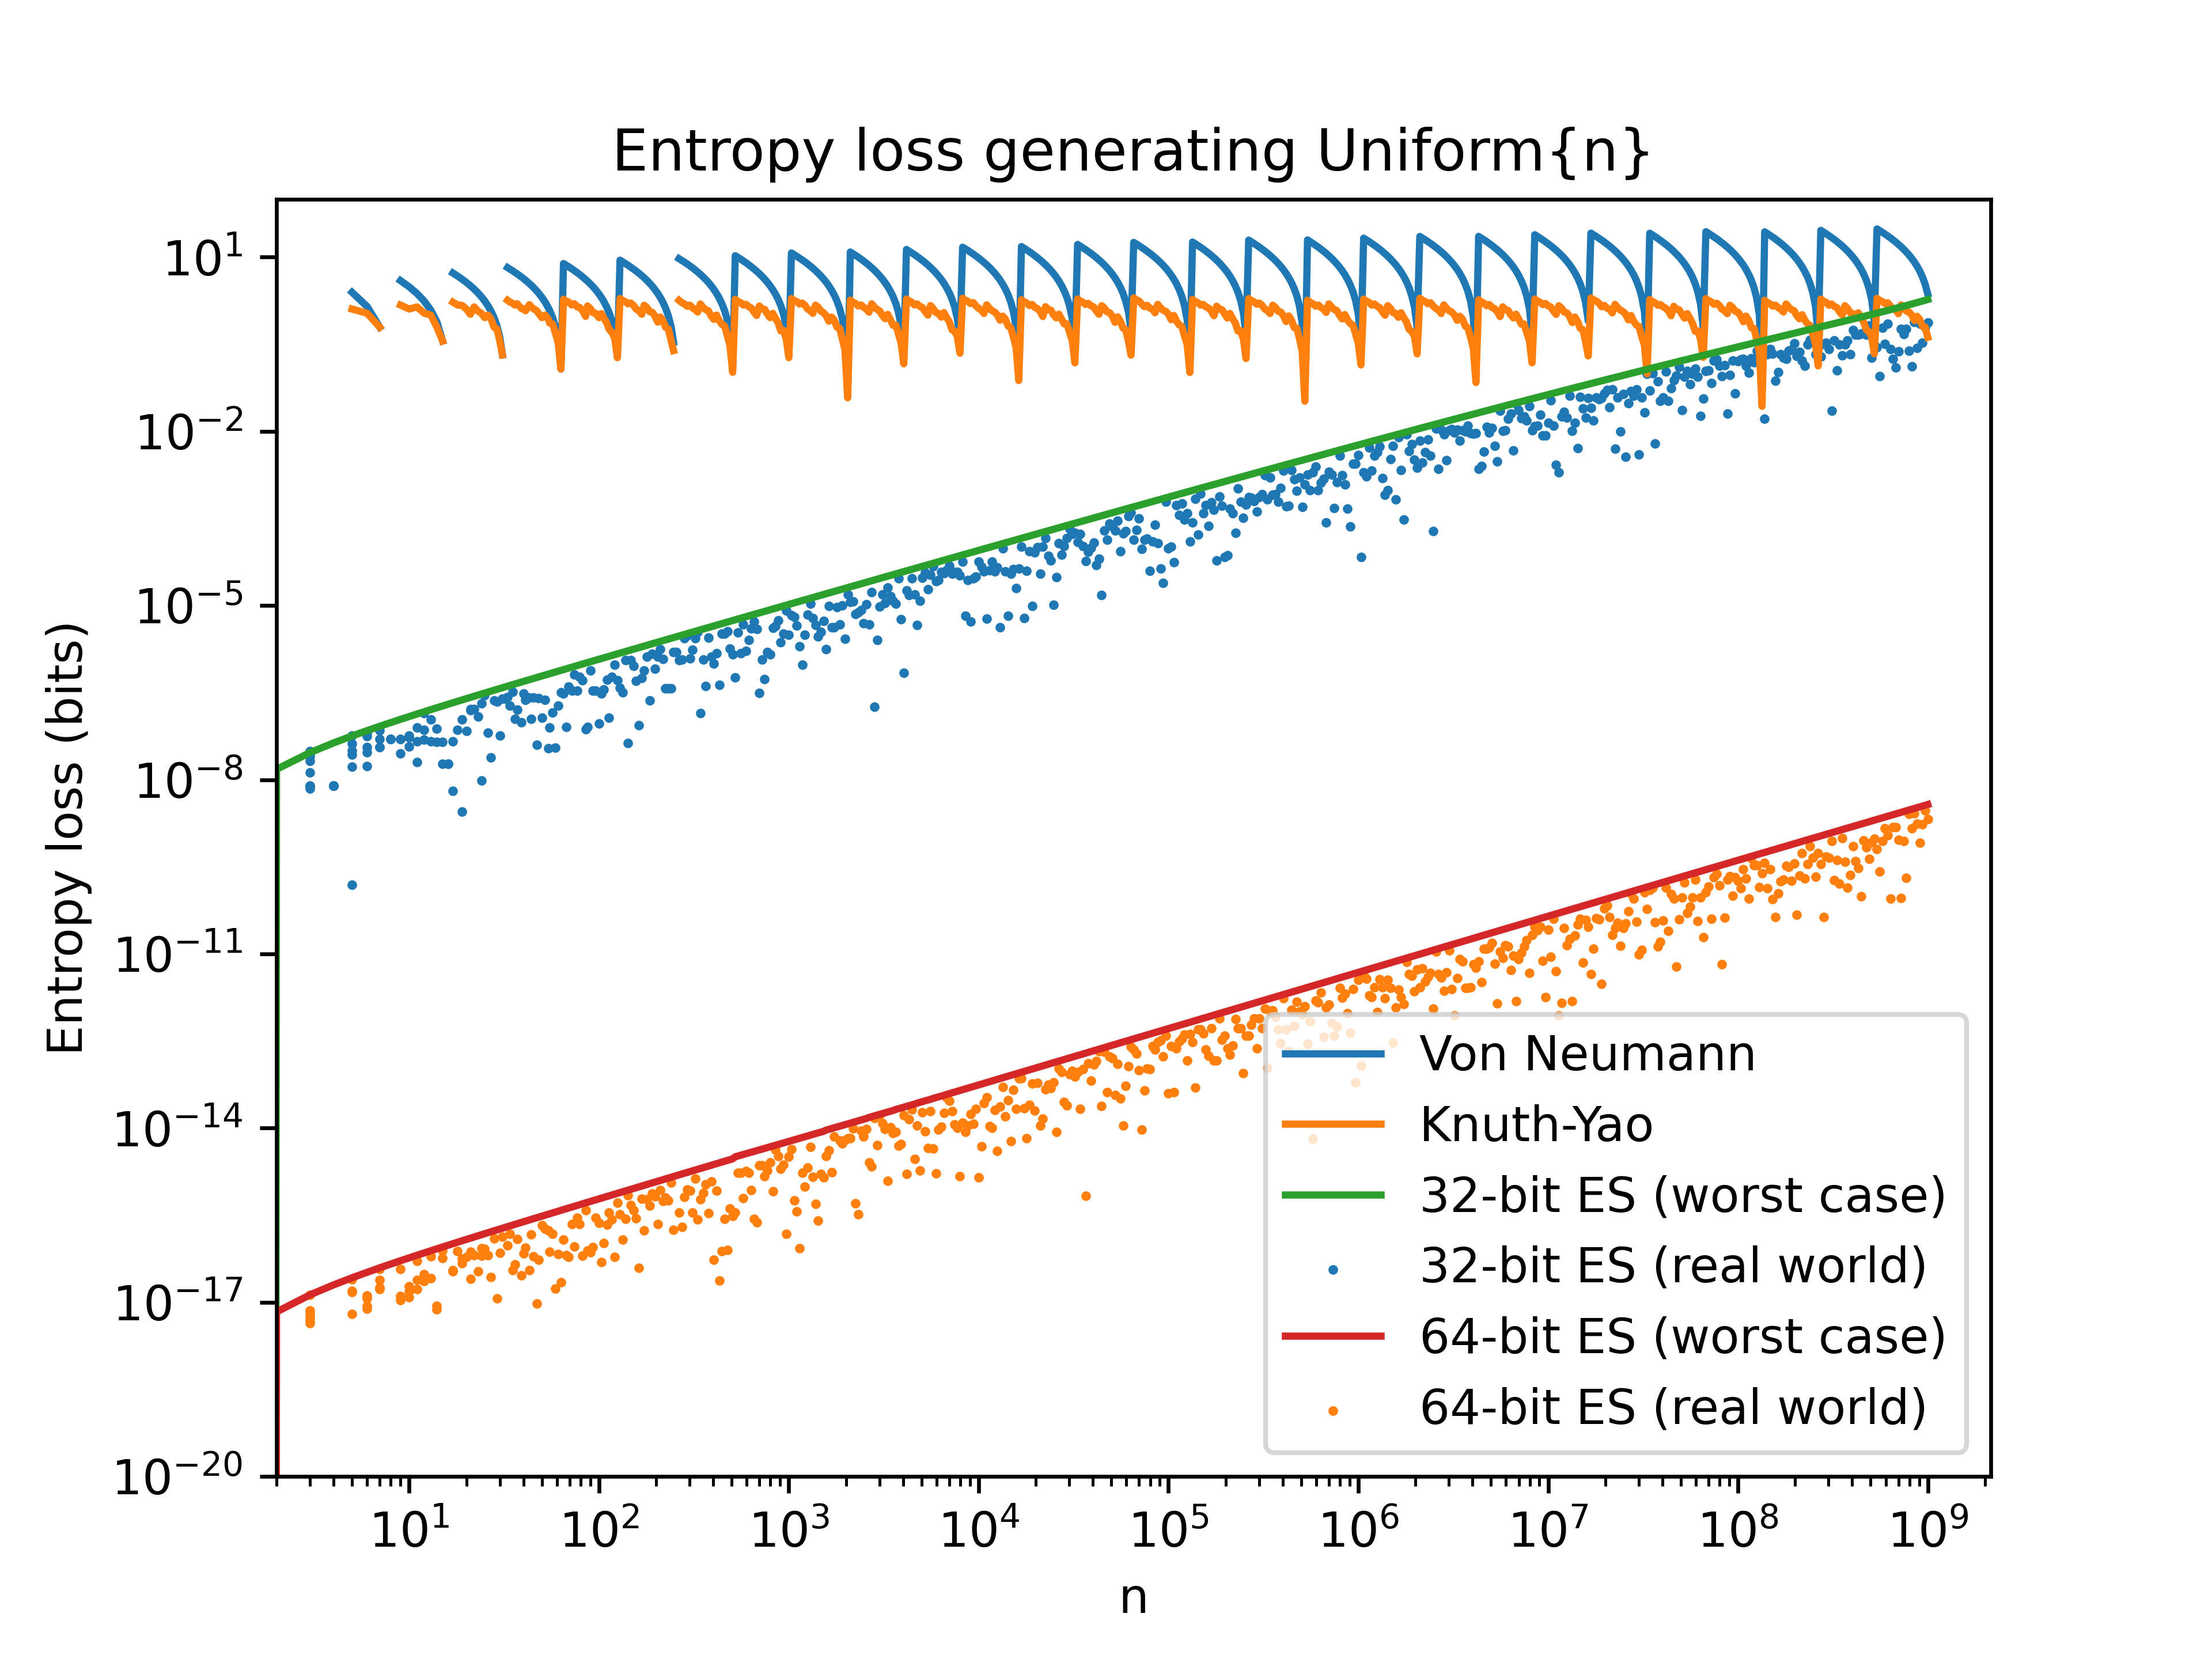
\includegraphics[width=0.8\textwidth]{uniform_losses.png}
\caption{Entropy losses for uniform variable generation.}
\label{fig:uniform-losses}
\end{figure}

Figure \ref{fig:shuffling-efficiency} shows the overall impact of entropy losses when applied to the shuffling a deck of $n$ cards using the Fisher-Yates algorithm \cite{fisher1953statistical, durstenfeld1964algorithm, knuth2014art}. This is a good demonstration of the entropy efficiency under a real-world workload. Calculations show that we can calculate that shuffling a deck of 52 cards can be done with an entropy loss of $\approxeq 1.7e-5$ bits, or an entropy efficiency of $\approxeq 0.99999992$.

\begin{figure}[ht]
\centering
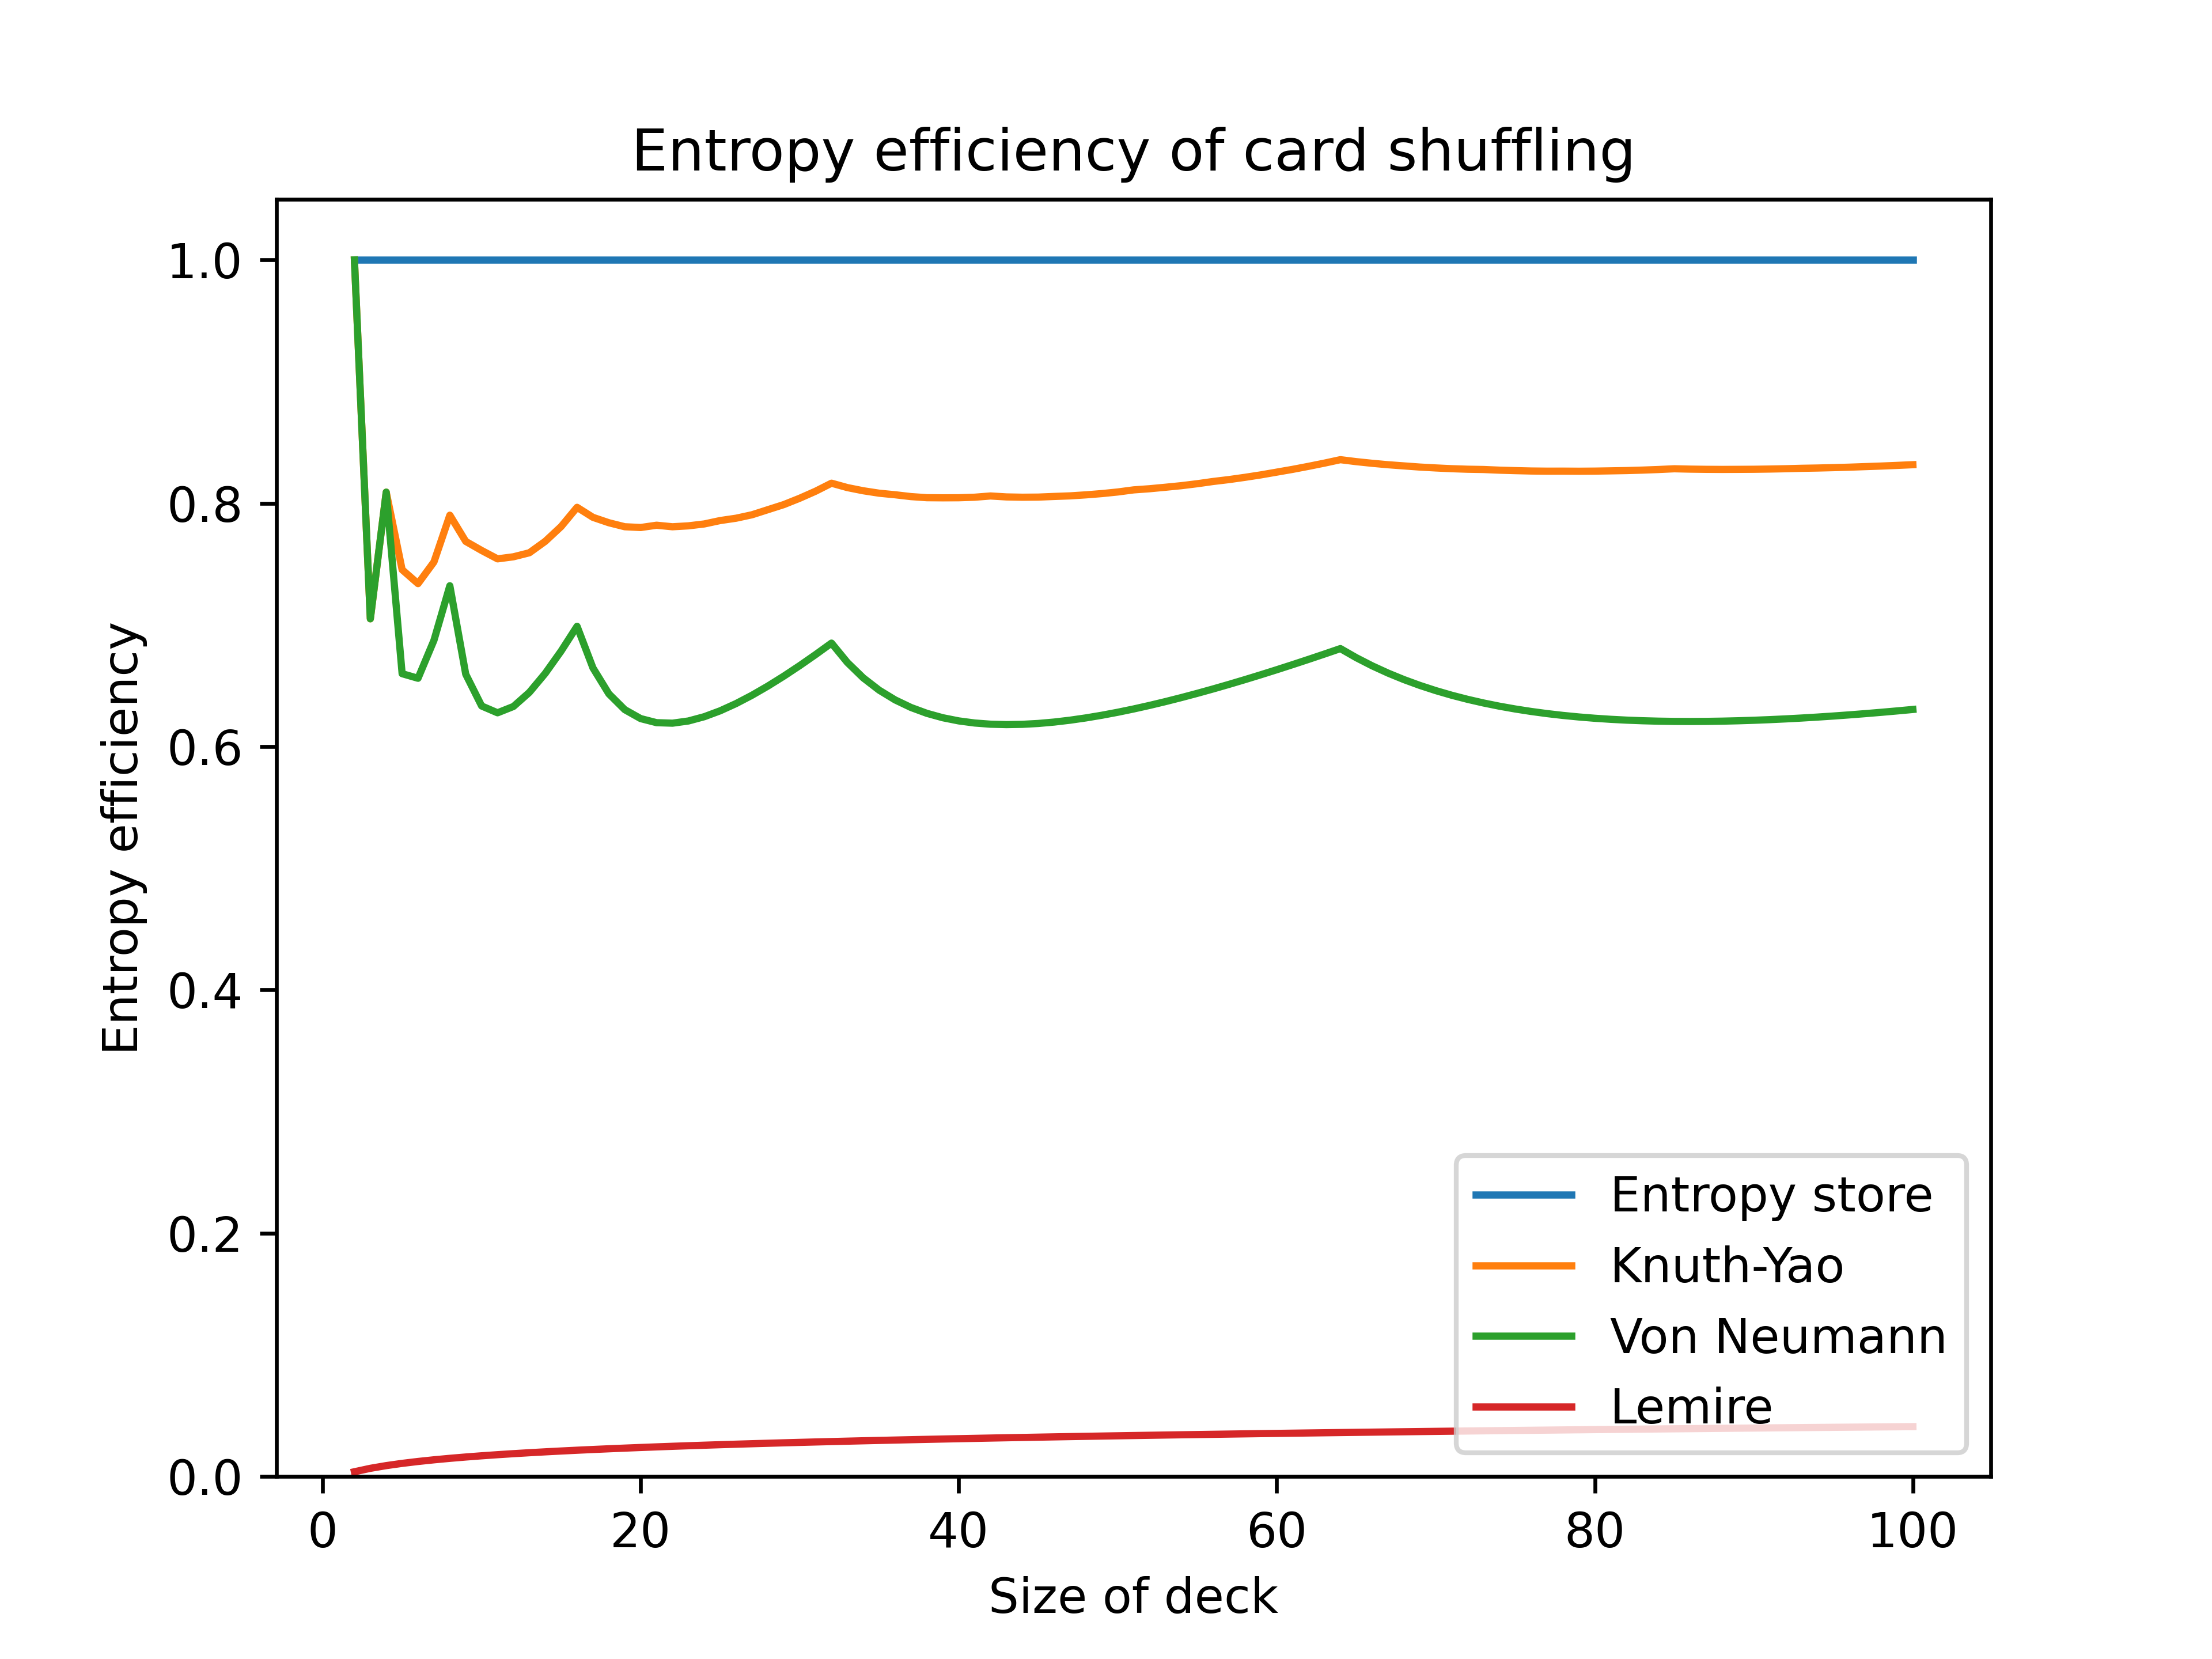
\includegraphics[width=0.8\textwidth]{shuffling_efficiency.png}
\caption{Entropy efficiency shuffling cards.}
\label{fig:shuffling-efficiency}
\end{figure}

When generating Bernoulli variables, we see in Figure \ref{fig:bernoulli-efficiency} that the entropy efficiency of the interval algorithm drops off significantly at lower entropy. Notice the "hair" on the $\bern{\frac{n}{1024}}$ line due to dyadic points being more efficient to generate with the IA. IA must fetch between 1 and 2 bits per output on average. By contrast, ES algorithms to not necessarily fetch any bits to generate an output, as there may be enough entropy in the store already, so ES just shrinks the size of its store to generate an output. Figure \ref{fig:bernoulli-rate} shows that IA cannot significantly increase its output rate for low-entropy outputs.

\begin{figure}[ht]
\centering
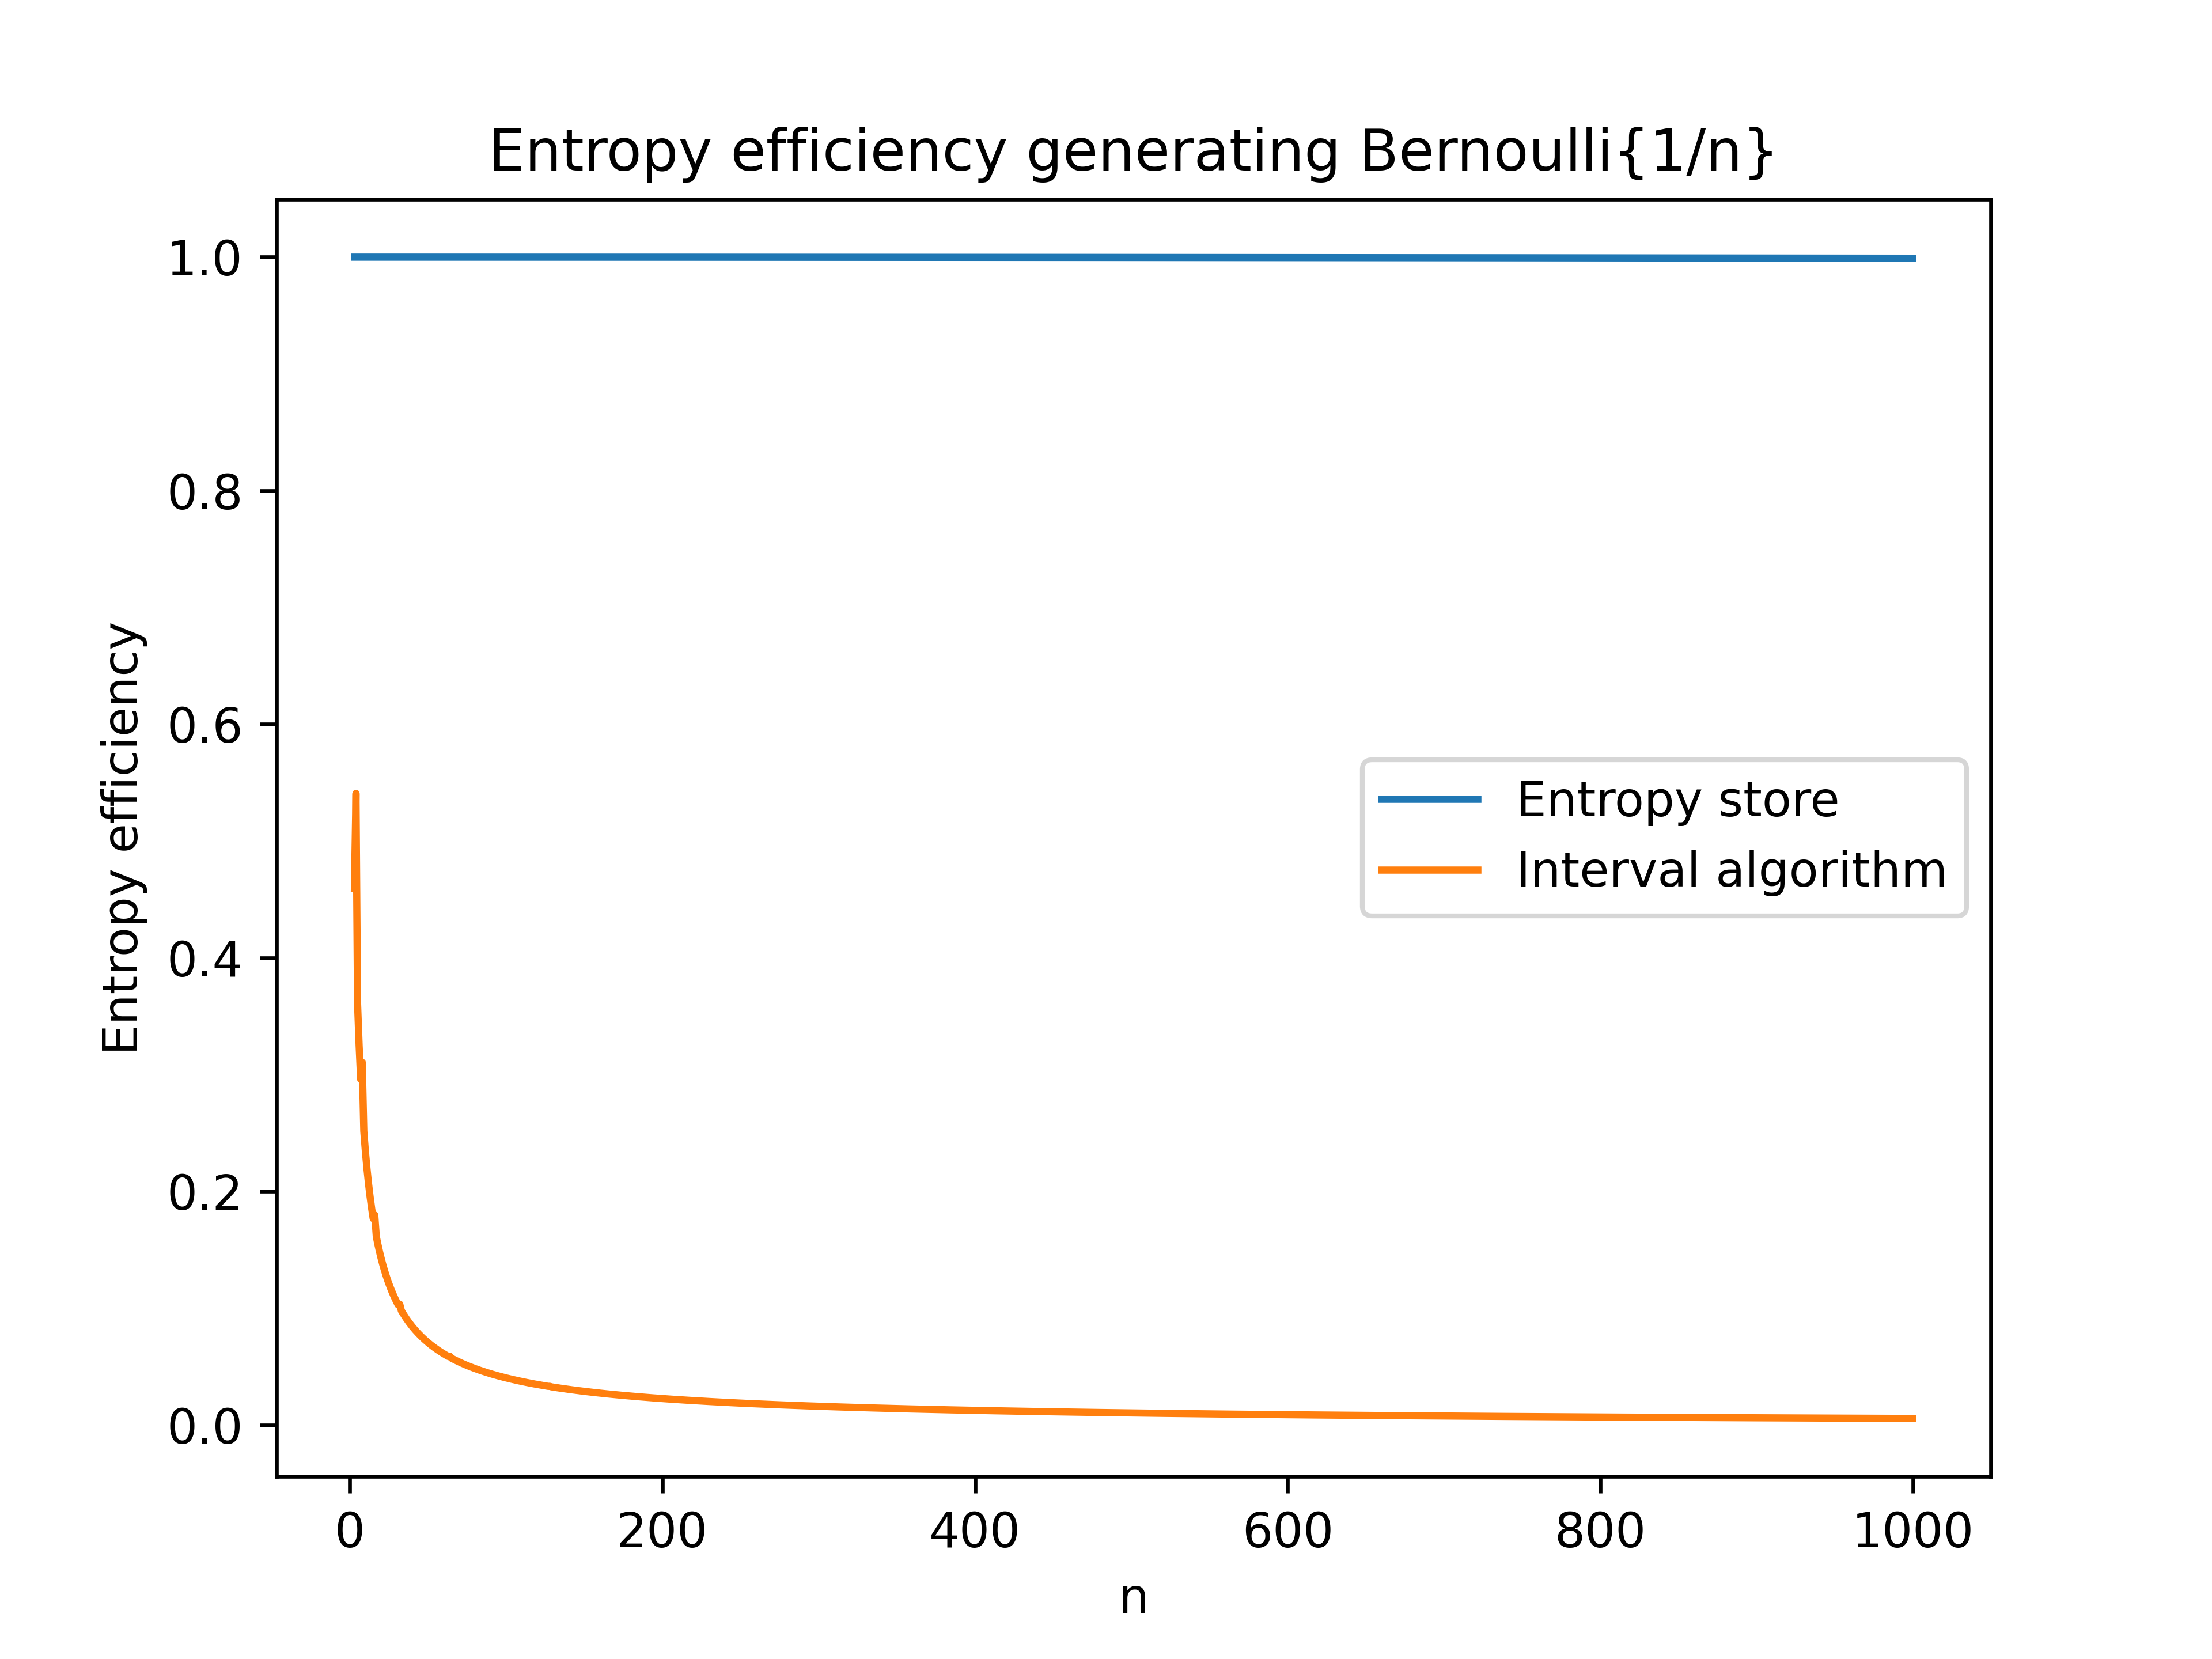
\includegraphics[width=0.8\textwidth]{bernoulli_efficiency.png}
\caption{Entropy efficiency generating Bernoulli variables.}
\label{fig:bernoulli-efficiency}
\end{figure}

\begin{figure}[ht]
\centering
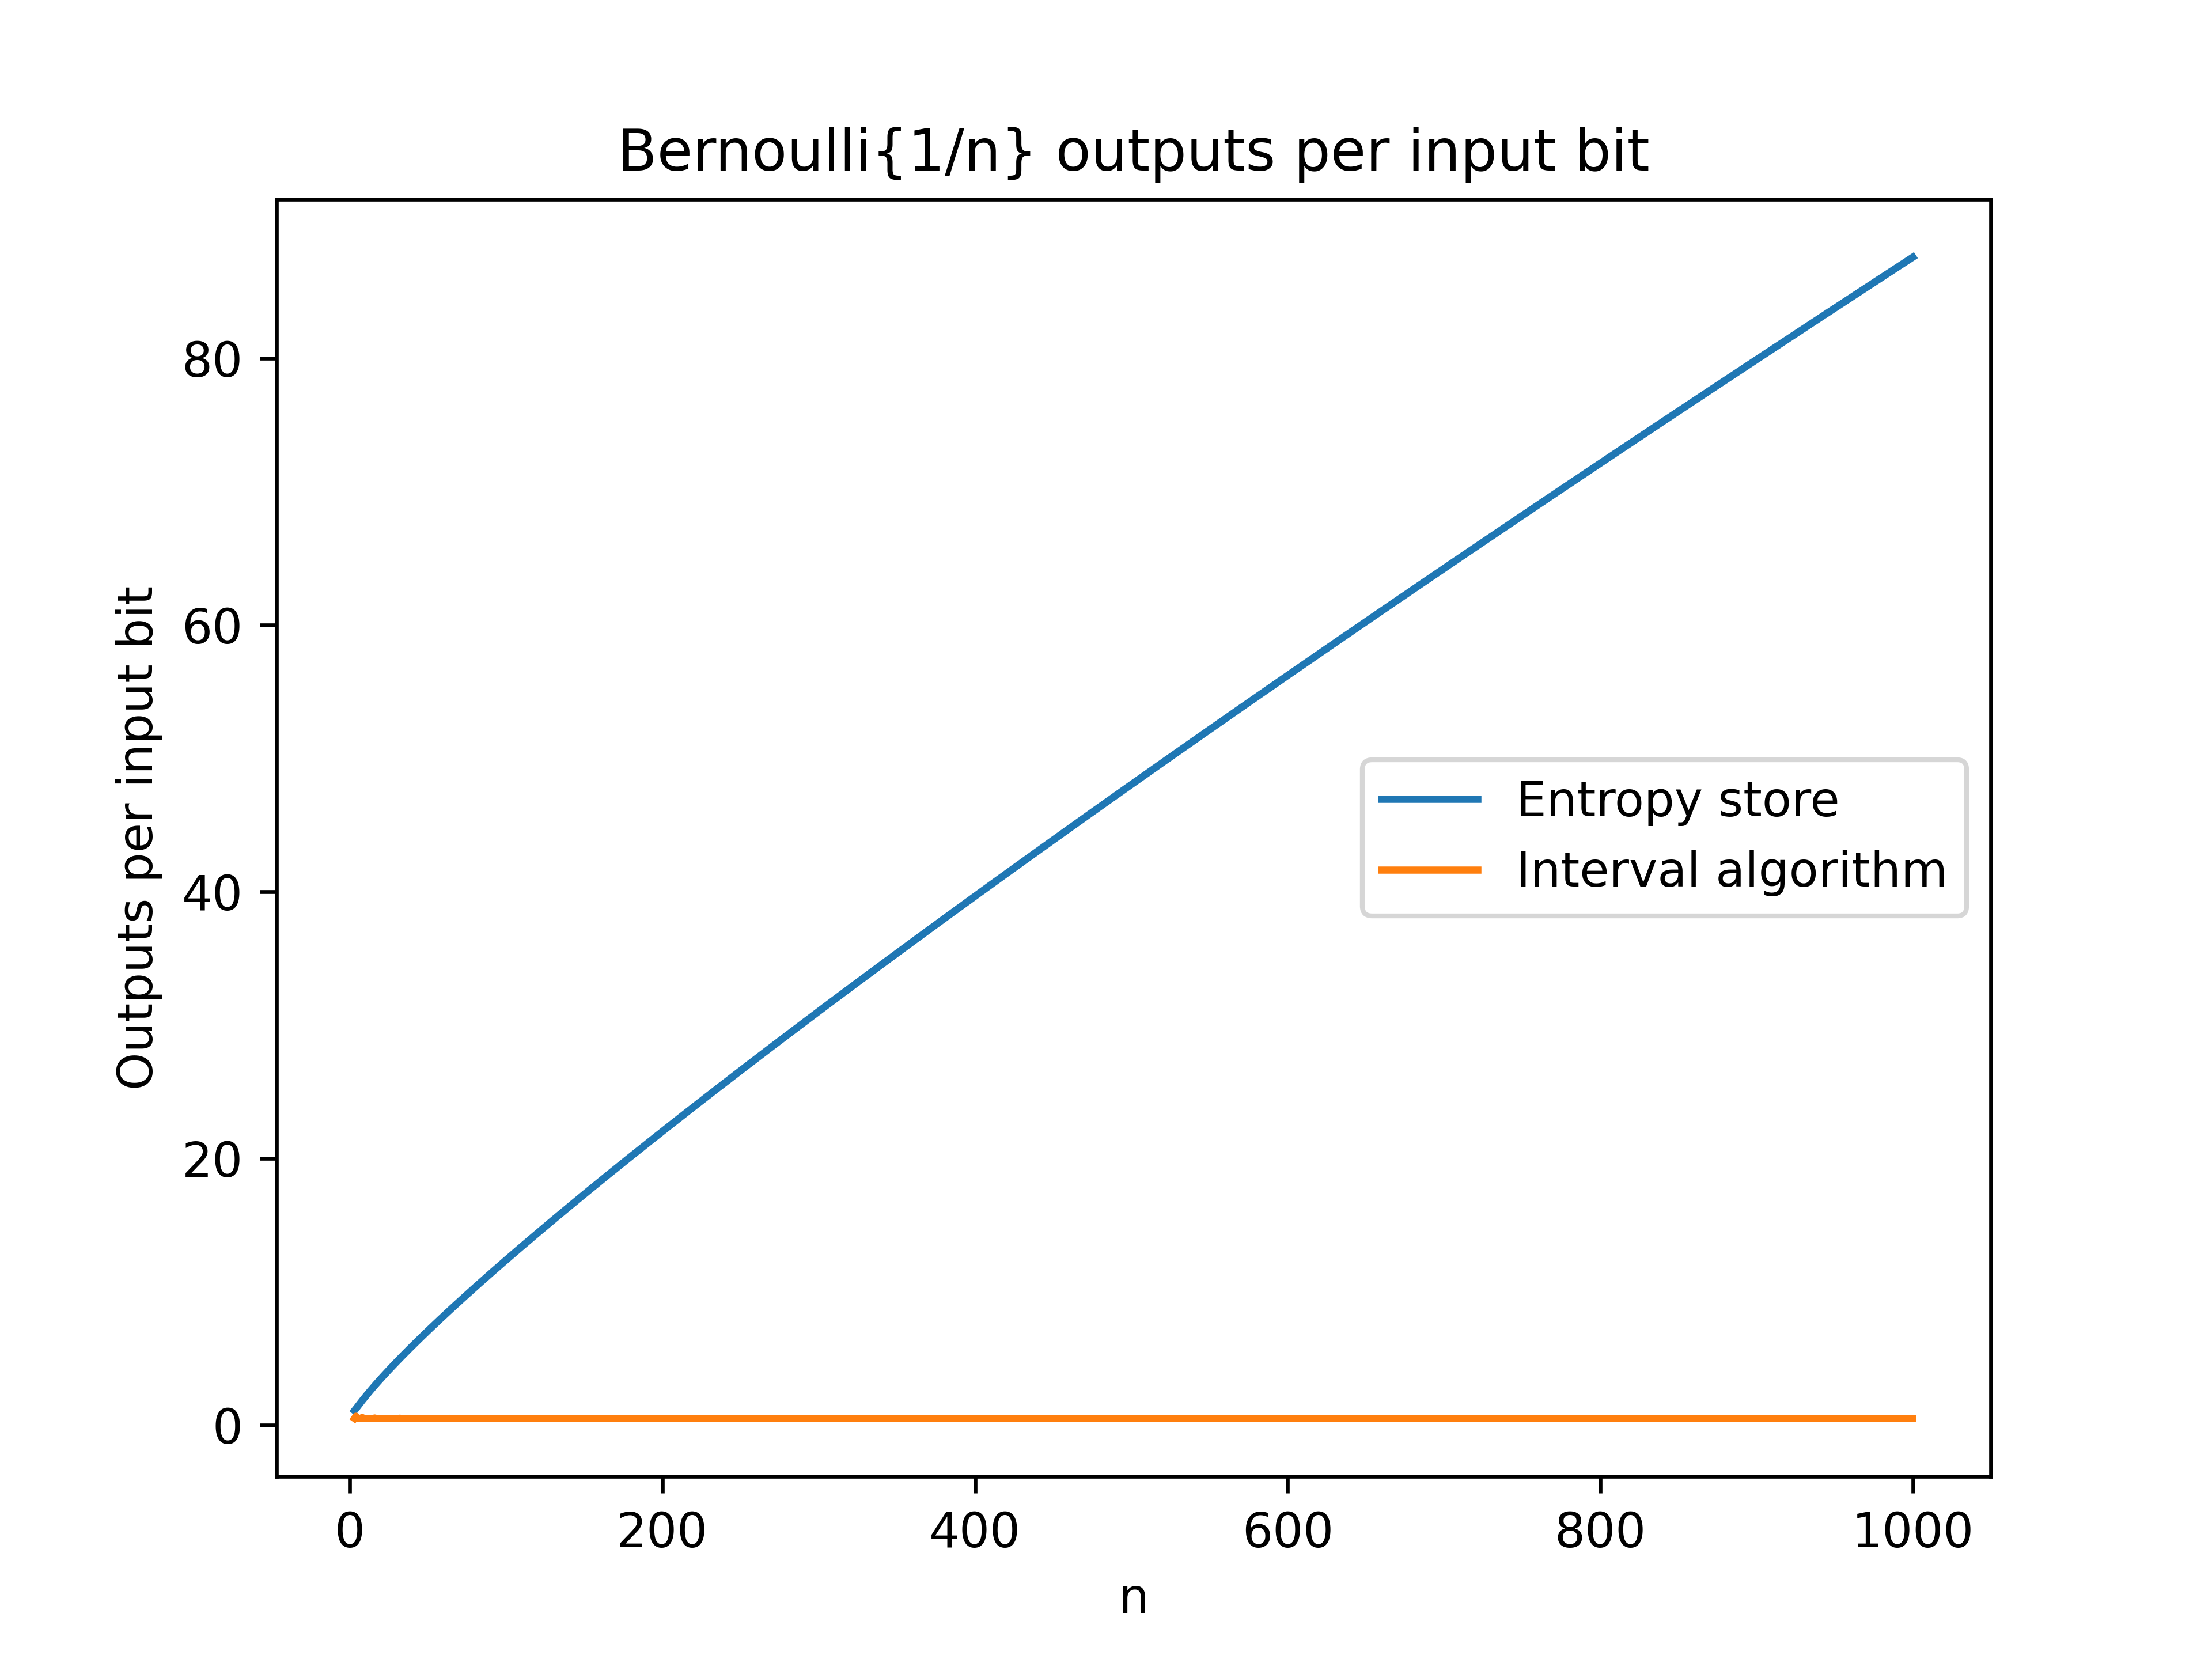
\includegraphics[width=0.8\textwidth]{bernoulli_rate.png}
\caption{Output rate for Bernoulli distributions.}
\label{fig:bernoulli-rate}
\end{figure}

Table~\ref{tab:speed} compares the speed of ES against various best in class random number generators. These numbers are heavily compiler and CPU dependent, so should not be taken too seriously.

When reading entropy from a hardware random generator, rate of entropy input is the dominating factor and the ES is the fastest by a significant margin. When using a very fast pseudo-random source like Xorisho-128 \cite{blackman21}, we see that Lemire's algorithm \cite{lemire2019fast} dominates, as this is designed for speed and not entropy-efficiency.

Speed is best understood in terms of CPU pipeline architecture. Branching, memory access, hardware random numbers and integer divmod operations are all relatively expensive operations \cite{Abel19a}. Table-based methods like FLDR \cite{saad2020fldr} and ALDR \cite{saad2025} perform memory access which can be slower than purely arithmetic methods. ES is likely to suffer due to its 2 integer divmod operations, but compilers can strength-reduce integer division to a multiplication and a shift \cite{granlund94}, which is shown in the "optimized" version of these algorithms in Table~\ref{tab:speed}. ES was fastest for Bernoulli outputs in all cases because there is only one division operation needed per output.

Overall, ES is most suited when generating truly random variables from a hardware entropy source. When a pseudo-random source is used, then Lemire's algorithm is the fastest. Using a 64-bit ES was detrimental because the consumed entropy does not significantly change, but the operations are slower.

Integer division and multiplication is $O(n \log n)$ \cite{harvey2021integer}, so for an $m$ bit ES the complexity is $O(m \log m)$, but for practical purposes it is $O(1)$ in time and space per output.

\begin{table}[h!]
\centering
\begin{tabular}{|c|c|c|c|}
\hline
Algorithm & Output & Hardware & Xoshiro-128++ \\
\hline
ES32                  & $\unif{6}$ & 1 & 1 \\
ES32 optimized        & $\unif{6}$ & 1 & 0.47 \\
ES64                  & $\unif{6}$ & 1 & 1.24 \\
ES64 optimized        & $\unif{6}$ & 1 & 0.55 \\
Von Neumann \cite{neumann51}     & $\unif{6}$ & 1.55 & 0.77 \\
Fast Dice Roller \cite{lumbroso2013optimal} & $\unif{6}$ & 1.42 & 0.83 \\
Huber-Vergas \cite{huber2024optimalrollingfairdice} & $\unif{6}$ & 1.42 & 1.0 \\
FLDR \cite{saad2020fldr} & $\unif{6}$ & 1.42 & 1.46 \\
ALDR \cite{saad2025} & $\unif{6}$ & 1.42 & 1.5 \\
Lemire \cite{lemire2019fast} & $\unif{6}$ & 24.8 & 0.26 \\
\hline

ES32                  & $\bern{\frac{1}{100}}$ & 1 & 1 \\
ES32 optimized        & $\bern{\frac{1}{100}}$ & 0.9 & 0.54 \\
FLDR                  & $\bern{\frac{1}{100}}$ & 28.3 & 3.8 \\
ALDR                  & $\bern{\frac{1}{100}}$ & 22.4 & 2.94 \\

\hline

ES32                  & $\mathrm{Weighted}\{1,2,3,4,5\}$ & 1 & 1 \\
FLDR                  & $\mathrm{Weighted}\{1,2,3,4,5\}$ & 1.36 & 1.38 \\
ALDR                  & $\mathrm{Weighted}\{1,2,3,4,5\}$ & 1.36 & 1.13 \\

\hline

\end{tabular}
\caption{Relative times generating integers from different binary entropy sources (lower is better).}
    \label{tab:speed}
\end{table}



\section{Conclusion}

We have introduced a new class of algorithm to generate random variables via a uniform entropy store, and shown that by recycling unused entropy between outputs we can achieve arbitrarily low entropy losses. We have shown that the entropy efficiency limits of classical algorithms like Knuth-Yao and the Interval Algorithm can be overcome by using an entropy store. 

A big benefit of ES is that no setup step is needed for uniform and Bernoulli outputs, and that the same ES can be shared between different output types. ES is fastest when generating outputs from a hardware entropy source and for Bernoulli outputs, but is still competitive on pseudorandom entropy sources, particularly if the division operations can be optimized.



\printbibliography

\appendix

\section {Source code} \label{app:source-code}

Source code for $\textsc{generate\_uniform}$, written in C.

\begin{verbatim}
    const uint32_t s_min = 1<<31;
    uint32_t s_value = 0, s_range = 1;

    uint32_t generate_uniform32(uint32_t n)
    {
        for(;;)
        {
            // Preload entropy one bit at a time into s
            while(s_range < s_min)
            {
                s_value <<= 1;
                s_value |= fetch();
                s_range <<= 1;
            }
            // Sample entropy s to a multiple of n
            uint32_t r = s_range / n;
            uint32_t m = s_range % n;
            if(s_value >= m)
            {
                // Sample successful
                s_value -= m;
                uint32_t a = s_value / n;
                uint32_t b = s_value % n;
                s_value = a;
                s_range = r; 
                return b;
            }
            else
            {
                // Reject
                s_range = m;
            }
        }
    }
\end{verbatim}

\end{document}
